\section{Improving Convergence Speed}

A good optimization algorithm is esential for fitting a deep neural network, however the convergence rate can often be improved by modifying the network aritecture itself such that the cost function is easier to optimize. These modifications does not radically alter the network, but rather modifies existing layers. The modifications can also become the idendity function though parameter optimization and thus doesn't change the theoretical capabilities of the neural network.

\subsection{Batch Normalization}
Traditionally in feed forward neural networks it has been the norm to standarize the input to have zero mean and unit variance.
\begin{equation}
\hat{x}_i = \frac{x_i - \mathbb{E}[x_i]}{\sqrt{\textsc{Var}[x_i]}}, \quad \forall i \in [1, I]
\end{equation}

This standaridization places the input to the sigmoid activation function in its linear domain ($\sigma(\epsilon) \approx \epsilon, \forall \epsilon \in [-1, 1]$), which is a reasonable starting point for the optimization \todo{[LeCun et al., 1998b; Wiesler \& Ney, 2011]}. Batch normalization extends this idea to standardize before all activation functions in a deep neural network. This has positive consequences beound limiting the sigmoid activation to its linear domain \cite{batch-normalization}.

Consider a neural network with just one hidden layers:
\begin{equation}
\mathcal{L}(\mathbf{t}, \mathbf{W}_2 \sigma(\mathbf{W}_1 \mathbf{x} + \mathbf{b}_1) + \mathbf{b}_2)
\end{equation}
where $\sigma$ is the activation function. When optimizing the loss function, the parameters $\mathbf{W}_1, \mathbf{W}_2, \mathbf{b}_1$ and $\mathbf{b}_2$ are all optimized simultaneously. Futhermore the optimization of $\mathbf{W}_2, \mathbf{b}_2$ does directly depend on $\sigma(\mathbf{W}_1 \mathbf{x} + \mathbf{b}_1)$ though the error term. This becomes and issue when the distribution of $\sigma(\mathbf{W}_1 \mathbf{x} + \mathbf{b}_1)$ changes, because the updated $\mathbf{W}_2$ and $\mathbf{b}_2$ assumes the original distribution. This change of the distribution of the internal activations is called an \textit{internal covariate shift}. \cite{batch-normalization}.

The \textit{internal covariate shift} issue can be ilustrated by considering a scalar $a = w x + b \sim \mathcal{N}(b, w)$, as it would appear in a very simple neural network, the sigmoid activation function is the applied on $\mathcal{N}(b, w)$ by using the \textit{change of variable theorem}. Using this one can change $w$ and $b$ and observe how the sigmoid activation distribution changes (Figure \ref{fig:batch-norm-activation-distribution}).

\begin{figure}[h]
	\centering
	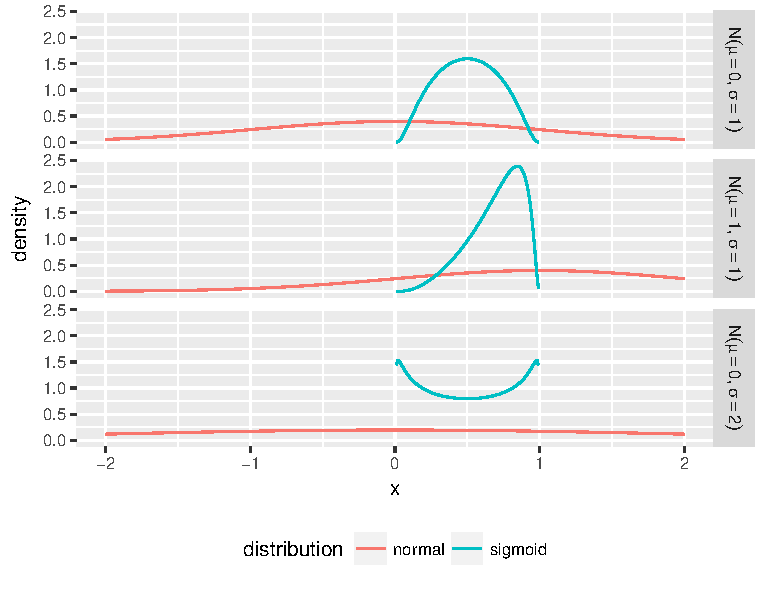
\includegraphics[scale=1]{theory/batch-norm-activation-distribution}
	\caption{Shows $X \sim \mathcal{N}(\mu, \sigma)$ and $\mathrm{sigmoid}(X)$ calculated using the \textit{change of variable theorem}.}
	\label{fig:batch-norm-activation-distribution}
\end{figure}

\subsubsection{A solution}
The \textit{internal covariate shift} issue can in practis be solved by using a small learning rate, however this is not an optimal solution as it prolongs the optimization. Batch Normalization is an alternative solution, that solves the issue by standardizing the input to the activation function. To truly standardize this input the convariance matrix, as well as its inverse square root should be calculated, this is very expensive thus Batch Normalization makes a pratical compromise by only standardizing using the variance.
\begin{equation}
\hat{z}_{h_\ell} = \frac{z_{h_\ell} - \mathbb{E}[z_{h_\ell}]}{\sqrt{\textsc{Var}[z_{h_\ell}]}}, a_{h_\ell} = \sigma(\hat{z}_{h_\ell})
\end{equation}

The expectation ($\mathbb{E}[z_{h_\ell}]$) and variance ($\textsc{Var}[z_{h_\ell}]$) themself are expensive to estimate over the entire dataset, thus it's only done over each mini-batch. This also makes it much more feasable to integrate the standardization into the backward pass. Note also that because the expectation is substracted, the bias $b_{h_\ell}$ in $z_{h_\ell}$ has no effect and should thus be obmitted:
\begin{equation}
z_{h_\ell} = \sum_{h_{\ell-1}}^{H_{\ell-1}} w_{h_{\ell-1}, h_\ell} a_{h_{\ell-1}} 
\end{equation}


Finally to allow Batch Normalization to become the indendity function, two more parameters ($\gamma, \beta$) are added to the optimzation problem:
\begin{equation}
\hat{z}_{h_\ell} = \gamma_{h_\ell} \frac{z_{h_\ell} - \mathbb{E}[z_{h_\ell}]}{\sqrt{\textsc{Var}[z_{h_\ell}]}} + \beta_{h_\ell}, a_{h_\ell} = \sigma(\hat{z}_{h_\ell})
\label{eq:theory:convergence:batch-norm}
\end{equation}

The backward pass for learning ($w, \gamma, \beta$) is rather complicated, but computationally completely feasible as long as the mini-batch size is small. See Appendix \ref{appendix:backward-pass:batch-norm} for the backward pass.

\subsubsection{Inference}

With an establised backward pass, the network can esily be trained. However there is still an open question about how inference should be done.

The inference should be determinstic once training is done, thus the ideal solution would be to use the estimated expectation and variance from the entire training dataset in \eqref{eq:theory:convergence:batch-norm}. However because this calculation can be rather expensitve a more practial solution is to use a moving average. Lets denote $\sigma^2_{\mathcal{B}_i}$ and $\mu_{\mathcal{B}_i}$ as the variance and mean estimate after mini-batch $i$. Then in addition to the optimization of ($w, \gamma, \beta$), $\sigma^2_{\mathcal{B}_i}$ and $\mu_{\mathcal{B}_i}$ will also updated during training.
\begin{equation}
\begin{aligned}
\sigma^2_{\mathcal{B}_i} &= \lambda \sigma^2_{\mathcal{B}_{i-1}} + (1 - \lambda) \textsc{Var}[z_{h_\ell}] \\
\mu_{\mathcal{B}_i} &= \lambda \mu_{\mathcal{B}_{i-1}} + (1 - \lambda) \mathbb{E}[z_{h_\ell}]
\end{aligned}
\end{equation}

At inference $\hat{z}_{h_\ell}$ are then calculated using $\sigma^2_{\mathcal{B}_i}$ and $\mu_{\mathcal{B}_i}$.

\begin{equation}
\hat{z}_{h_\ell} = \gamma_{h_\ell} \frac{z_{h_\ell} - \mu_{\mathcal{B}_i}}{\sqrt{\sigma^2_{\mathcal{B}_i}}} + \beta_{h_\ell}, a_{h_\ell} = \sigma(\hat{z}_{h_\ell})
\end{equation}

\subsubsection{Weight sharing network}

Because it is the weight changes that causes an \textit{internal covariate shift}, the normalization should happen over all $z_{h_\ell}$ values that uses these weights. Thus in RNN the normalization should also be done over time, and in CNN the normalization should also happen over the ``image''. This works well for actual images, however in RNN and temporal CNN this breaks the causalily of the network, because the mean and variance at any time step (e.g. $t=0$) will contain information from all time steps.

\subsection{Layer Normalization}
\cite{layer-normalization}

\subsection{Residual Learning}
\cite{residual-learning}
